\documentclass[11pt]{article}
\input{\string~/.macros}
\usepackage[a4paper, total={7in, 9in}]{geometry}
\usepackage{bbm}
\usepackage{mathrsfs} % really cursive alphabets
\usepackage{graphicx}
    \graphicspath{{./assets}}
\usepackage{hyperref}
    \hypersetup{colorlinks=true, linktoc=all, linkcolor=blue, citecolor=red}
\usepackage[backend=bibtex,sorting=none]{biblatex}
\usepackage[margin=0cm]{caption}

% random variables
\newcommand\ry{\ensuremath{\mathsf{y}}}
\newcommand\rx{\ensuremath{\mathsf{x}}}
\newcommand\rb{\ensuremath{\mathsf{b}}} 
\newcommand\rc{\ensuremath{\mathsf{c}}}
\newcommand\rz{\ensuremath{\mathsf{z}}}
\newcommand\ru{\ensuremath{\mathsf{u}}}
\newcommand\rw{\ensuremath{\mathsf{w}}}
\newcommand\rpa{\ensuremath{\mathsf{pa}}}
\newcommand\rU{\ensuremath{\mathsf{U}}}
\newcommand\rbx{\ensuremath{\mathsf{\mathbf{x}}}}
\newcommand\rby{\ensuremath{\mathsf{\mathbf{y}}}}
\newcommand\rbu{\ensuremath{\mathsf{\mathbf{u}}}}

\newcommand\bbP{\ensuremath{\mathbbm{P}}}
\newcommand\bbQ{\ensuremath{\mathbbm{Q}}}


% boldsymbols
\renewcommand\bmu{\ensuremath{\boldsymbol{\mu}}}
\newcommand\bSigma{\ensuremath{\boldsymbol{\Sigma}}}
\newcommand\bgamma{\ensuremath{\boldsymbol{\gamma}}}
\newcommand\bomega{\ensuremath{\boldsymbol{\omega}}}
\newcommand\bnu{\ensuremath{\boldsymbol{\nu}}}


% optimization, classes of functions
\newcommand\scrF{\ensuremath{\mathscr{F}}}
\newcommand\scrS{\ensuremath{\mathscr{S}}}
\newcommand\scrP{\ensuremath{\mathscr{P}}}

% independence
\newcommand{\dperp}{\ensuremath{\perp\!\!\!\perp}}
\newcommand{\ndperp}{\ensuremath{\not\!\perp\!\!\!\perp}}

% operators
\newcommand{\prox}{\ensuremath{\mathsf{prox}}}
\addbibresource{kernel.bib}

\begin{document}
 
\section{Support Vector Machines}
 
Support vector machine is a kernelized optimal margin linear classifier (original paper \cite{boserTrainingAlgorithmOptimal1992} and a nice summary \cite{vertPrimerKernelMethods2004}). It distinguishes itself from classifiers minimizing empirical risk as it favors classifier which makes confident predictions. For binary classification problem $\sY=\pc{-1,+1}$, we are interested in finding a linear decision bondary, parameterized by $w\in\R^d,b\in\R$, that separates the training data points by maximizing the worst case distance (margin) of each data point to the decision boundary. We first assume that training set can be linearly separated. Given dataset $\pc{(x_i,y_i)}_{i=1}^n$, we are interested in solving the following quadratic programming problem,
\begin{align*}
    \min_{w,b}
        \;& \frac{1}{2} \norm{w}^2 \\
    \text{s.t.}
        \;& y_i(w^Tx_i + b) \geq 1 \quad i=1,2,\cdots,n
\end{align*}
To derive the dual problem, we write the Lagrangian, 
\begin{align}
    \sL(w,b,\alpha)
        &= \frac{1}{2} \norm{w}^2 + \sum_{i=1}^n \alpha_i \pb{ 1 - y_i(w^Tx_i+b) }
\end{align}
where $\alpha = \pc{\alpha_i}_{i=1}^n$ are the dual variables. Solve for $\inf_{w,b} \sL(w,b,\alpha)$ to arrive at the dual objective. In particular, first order optimality condition gives $w = \sum_{i=1}^n \alpha_i y_i x_i$ and it must be that $0=\sum_{i=1}^n \alpha_i y_i$. Therefore, 
\begin{align*}
    \max_{\alpha}
        \;& \sum_{i=1}^n \alpha_i - \frac{1}{2} \sum_{i=1}^n\sum_{j=1}^n \alpha_i \alpha_j y_i y_j x_i^Tx_j \\
    \text{s.t.}
        \;& \alpha_i \geq 0 \quad i=1,2,\cdots, n
            \tag{dual feasibility} \\
        & \sum_{i=1}^n \alpha_i y_i = 0 
            \tag{from $\nabla_b \sL = 0$}
\end{align*}
The dual can be solved more efficiently than the primal problem using coordinate descent. The decision rule is linear w.r.t support vectors (those $x_i$ right on margin with $\alpha_i > 0$)
\begin{align}
    \hat{y}(x) = \text{sgn}\left(
        \sum_{i=1}^n \alpha_i y_i x_i^T x + b
    \right)
    \quad\text{for}\quad
    b 
        = y_i - \sum_{j=1}^n \alpha_j y_j x_j^T x_i
\end{align}
for any support vector $x_i$. We observe that optimization as well as prediction uses input vectors via dot products only. We are motivated to use feature mapping $\phi:\sX\to\sH$ to map input vectors to a higher dimensional possibly infinite feature space in hope that the lifted space is linearly separable. The kernel function $k: \R^d\times\R^d \to \R$ allows us to compute dot products $k(x_i,x_j)=\inner{\phi(x_i)}{\phi(x_j)}_{\sH}$ efficiently and represents a notion of similarity over two instance of aribtrary objects, e.g. vectors in $\R^n$, graphs, texts. We can substitute $k$ whenever inner product is used and arrive at a optimal margin classifier over implicitly defined nonlinear feature mapping $\phi$. In case when training dataset is not linearly separable, we can introduce slack variable $\pc{\xi_i}_{i=1}^n$ where $x_i\geq 0$ to relax the inequality constraints and penalize misclassified or within margin points with $C\sum_{i=1}^n \xi_i$ for some $C\in\R$. In this case, we have the following Lagrangian,
\begin{align}
    \sL(w,\xi,\alpha,\beta)
        = \frac{1}{2}\norm{w}^2 + C\sum_{i=1}^n \xi_i + \sum_{i=1}^n \alpha \left( 1-y_i ( \inner{w}{\phi(x_i)}_{\sH} + b )-\xi_i \right) + \sum_{i=1}^n \beta_i \xi_i
\end{align}
First order condition $0 = \frac{\partial}{\partial \xi_i}\sL = C - \alpha_i + \beta_i$ together with dual feasibility $\beta_i\geq 0$ yield $\alpha_i \leq C$ for all $i=1,2,\cdots,n$. Therefore, we optimize for the following dual problem,
\begin{align}
    \min_{\alpha}
        \;& \frac{1}{2} \alpha^T Q \alpha - 1^T \alpha  \\
    \text{s.t.}
    \;& y^T\alpha = 0 \\
    \;& 0\leq \alpha_i \leq C \quad i=1,2,\cdots, n
\end{align}
where $Q \in \R^{n\times n}$ with $Q_{ij} = \alpha_i \alpha_j k(x_i,x_j)$,
with optimal decision rule as
\begin{align}
    \hat{y}(x) = \text{sgn}\left(
        \sum_{i=1}^n \alpha_i y_i k(x_i,x) + b
    \right)
    \quad\text{for}\quad
    b = y_i - \sum_{j=1}^n \alpha_j y_j k(x_j,x_i)
\end{align}
for any support vector $i$, i.e. $0 < \alpha_i < C$.

\begin{center} 
\begin{figure}[h!]
    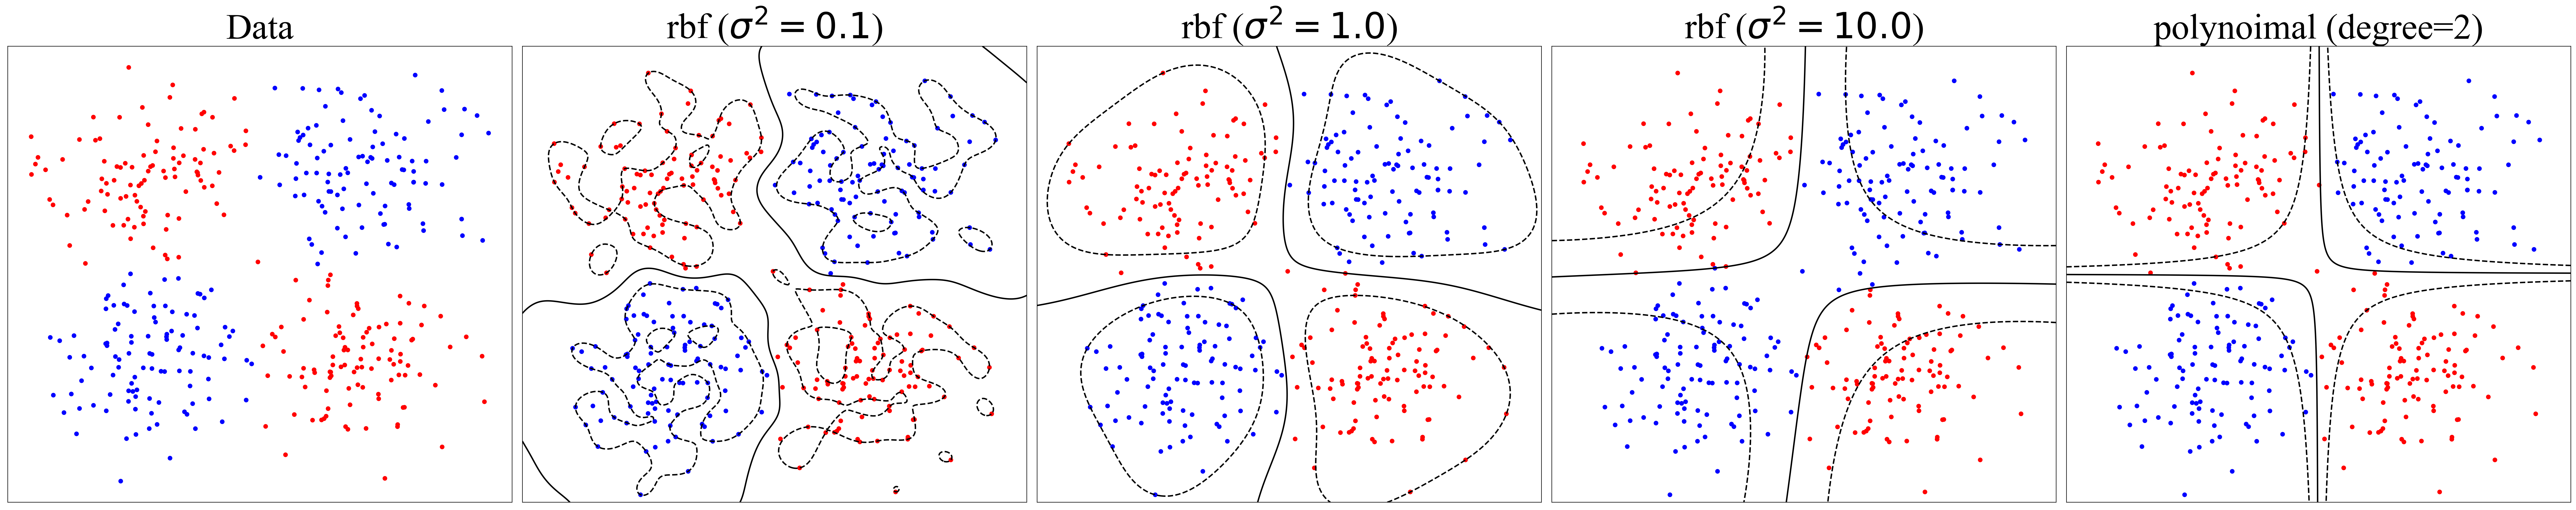
\includegraphics[width=\textwidth]{assets/svm_on_2d_gaussian_vary_kernel.png} 
    \caption{SVM on simulated 2D Gaussian with degree two polynomial kernel and radial basis function kernel with varying bandwidth. Larger bandwidth corresponds to smoother decision boundary and in the limit approaches the decision boundary of a linear kernel}
\end{figure}
\end{center} 
 

\section{Reproducing Kernel Hilbert Space}

\cite{grettonWhatRKHS2012} provides a rigorous introduction to RKHS while \cite{grettonIntroductionRKHSSimple2019} provides pretty good intuitions. 
Intuitively, RKHS can be considered as (1) a space of well-behaved functions whose smoothness is determined by its kernel. This view is useful when trying to think about regularization in terms of $\norm{f}_{\sH}^2$ (2) an inner product space for features. This view is useful when trying to apply kernel trick. (3) a space of functions spanned by representors $\pc{k(x,\cdot)}_{x\in\sX}$. We think of functions in RKHS as a simple function class, i.e. linear with respect to $\phi(x)$, and also flexible due to various choice of kernels. (4) a space of functions spanned by countably many eigenfunctions of the integral operator of kernel.


\begin{figure}[h!]
\begin{center}
    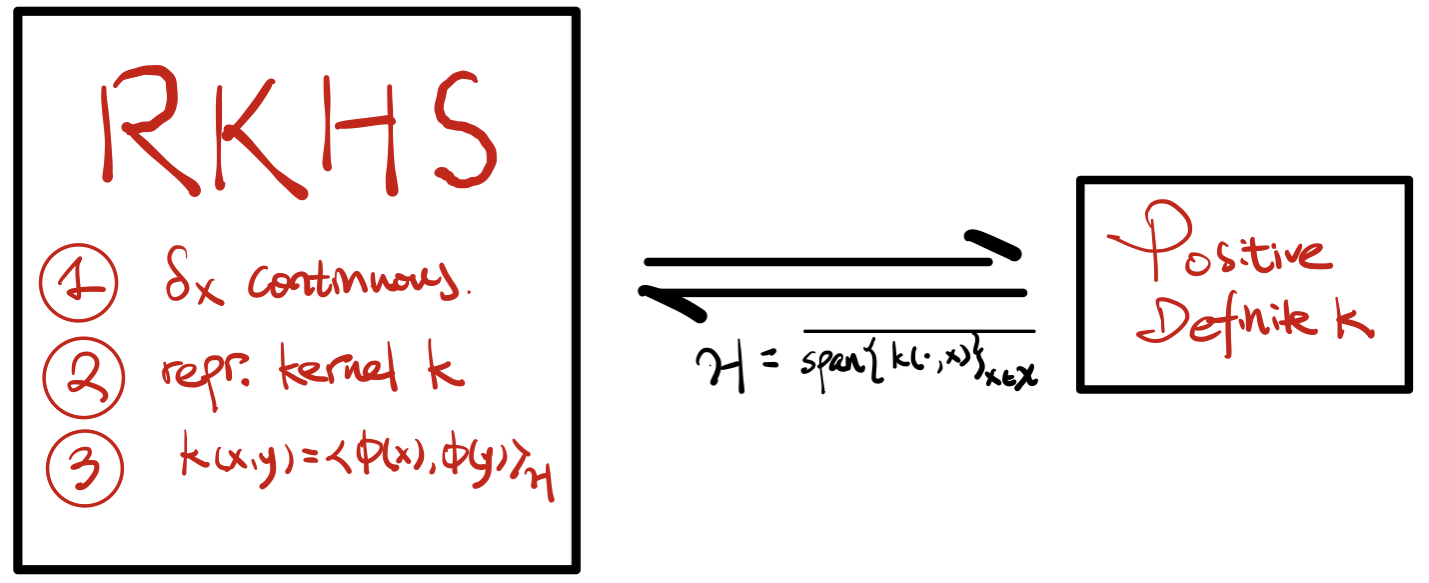
\includegraphics[height=3cm]{assets/rkhs_equivalence_schematics} 
    \caption{Equivalent views of RKHS}
\end{center}
\end{figure}


\begin{definition}
    (Hilbert space) A Hilbert space is a complete inner product space, i.e. $(\sH, \inner{\cdot}{\cdot}_{\sH})$
\end{definition}

\begin{definition}
    (Separable Hilbert space) A Hilbert space is separable if it has a countable basis
\end{definition}

\begin{definition}
    (Reproducing kernel Hilbert space) A Hilbert space $\sH$ of functions $f:\sX\to\R$ is a RKHS if its evaluation functional, $\delta_x:\sH\to\R$ where $\delta_x(f) = f(x)$ is continuous $\forall x\in\sX$.
\end{definition}

Intuitively, RKHS is a space of well-behaved functions. In particular, norm convergence in $\sH$ yield pointwise convergence, i.e. $\lim_{n\to\infty}\norm{f_n-f} = 0$ implies $f_n \to f$. Note evaluation functional is linear. The condition that $\delta_x$ is continuous is equivalent to $\delta_x$ be bounded \cite{grettonWhatRKHS2012}. Regularization of the form $\norm{f}_{\sH}$ leads to regularization on function values.

\begin{definition}
    (Reproducing kernel) Let $\sH$ be Hilbert space defined on non-empty $\sX$, then a function $k:\sX\times\sX\to\R$ is called a reproducing kernel of $\sH$ if
    \begin{enumerate}
        \item $\forall x\in\sX$, $k(x,\cdot)\in\sH$ 
        \item $\forall x\in\sX$, $\forall f\in\sH$, $f(x) = \inner{f}{k(x,\cdot)}_{\sH}$ (reproducing property)
    \end{enumerate}
    In particular, for any $x,y\in\sX$, $k(x,y) = \inner{k(y,\cdot)}{k(y,\cdot)}_{\sH}$.
\end{definition}

Intuitively, the definition of reproducing kernel implies that $k(x,\cdot)$ is (1) a high dimensional representer of $x$, and (2) as a representer of evaluation for any function in $\sH$ on data point $x$. We also note that we can always find a feature map associated with a reproducing kernel, namely the canonical feature map $\phi:x\to k(x,\cdot)$, and represent $k$ as an inner product in feature space $k(x,y) = \inner{\phi(x)}{\phi(y)}_{\sH}$. It turns out that RKHS has $\sH$ is a RKHS if and only if $\sH$ has a reproducing kernel. Definition of RKHS based on continuous evaluation functional is equivalent to existence of a (unique) reproducing kernel. 

\begin{definition}
    (Positive definite functions) A symmetric function $h:\sX\times\sX\to\R$ is positive definite if for all $n\geq 1$ and for all $(a_1,\cdots,a_n)\in\R^n$ for all $(x_1,\cdots,x_n)\in\sX^n$, 
    \begin{align}
        \sum_{i=1}^n \sum_{j=1}^n a_i a_j h(x_i,x_j) \geq 0
    \end{align}
\end{definition}
If you consider a function $k:\sX\times\sX\to\R$, $k$ is positive definite if any kernel matrix $K\in\R^{n\times n}$ where $K_{ij}=k(x_i,x_j)$ is positive definite, i.e. $K\succeq 0$. 

\begin{definition}
    (Kernel defined via feature map) Let $\sX$ be non-empty set. The function $k:\sX\times\sX\to\R$ is a kernel if there exists a real Hilbert space $\sH$ and a map $\phi:\sX\to\sH$ such that $\forall x,y\in\sX$, $k(x,y)=\inner{\phi(x)}{\phi(y)}_{\sH}$. $\phi$ is said to be the feature map and $\sH$  be the feature space.
\end{definition}

Note there maybe more than one feature map yield for any one kernel. Intuitively, a kernel is a function that can be represented as inner product. It turns out that RKHS with reproducing kernel $k$ is positive definite,
\begin{align}
    \sum_{i=1}^n \sum_{j=1}^n a_i a_j k(x_i,x_j)
        = \sum_{i=1}^n \sum_{j=1}^n a_i a_j \inner{k(x_i,\cdot)}{k(x_j,\cdot)}
        = \inner{\sum_{i=1}^n a_i \phi(x_i)}{\sum_{i=1}^n a_i \phi(x_i)}_{\sH}
        \geq 0
\end{align}
and, conversely, we can show that for every positive definite function $k$ there is an unqiue RKHS whose reproducing kernel is $k$ (Moore-Aronsajn). Intuitively, we construct a RKHS $\sH = \overline{\sH_0}$, the completion of a pre-RKHS space $\sH_0 = \text{span}(\pc{k(x,\cdot)}_{x\in\sX})$. In particular, the choice of inner product 
\begin{align}
    \inner{f}{g}_{\sH_0}
        = \sum_{i=1}^n\sum_{j=1}^m \alpha_i \beta_j k(x_i,y_j)
\end{align}
for $f = \sum_i \alpha_i k(x_i,\cdot), g = \sum_j \beta_j k(y_j,\cdot)$ makes $\sH_0$ a valid pre-RKHS. Intuitively, this construction implies that RKHS is a space spanned by representers $\pc{k(x,\cdot)}_{x\in\sX}$.



\begin{definition}
    (Integral Operator \cite{grettonWhatRKHS2012,muandetKernelMeanEmbedding2017}) Let $X$ be compact Hausdorff space and $\mu$ be finite Borel measure over $\sX$. Let $k$ be a continuous kernel. The integral operator of kernel $k$ is $T_k: L_2(\sX,\mu) \to L_2(\sX,\mu)$ defined 
    \begin{align}
        T_kf
            = \int_{\sX} k(x,\cdot) f(x) d\mu(x)
    \end{align}
\end{definition}

If $k$ is a positive definite function, then $T_k$ is self-adjoint ($\inner{f}{T_kg} = \inner{T_kf}{g}$ $\forall f,g\in L_2(\sX,\mu)$) positive ($\inner{f}{T_kf} \geq 0$ $\forall f\in L_2(\sX,\mu)$) and compact.

\begin{theorem}
    (Mercer's theorem) Assume $\sX,k,T_k$ defined as previous. Suppose for all $f\in L_2(\sX,\mu)$, we have $\int_{\sX} k(x,y) f(x)f(y) dxdy \geq 0$. Then there exists a countable orthonormal basis $\pc{e_i}$ of $L_2(\sX,\mu)$ consisting of eigenfunctions of $T_k$ whose corresponding eigenvalues $\pc{\lambda_i}$ are non-negative. Then,
    \begin{align}
        k(x,y)
            = \sum_{i=1}^{\infty} \lambda_i e_i(x) e_j(y)
    \end{align}
    for all $x,y\in\sX$. The convergence is absolute and uniform.
\end{theorem}

Mercer's theorem provides a construction of rkhs using eigenfunctions of integral operator. In particular $\sH = \pc{\sum_i a_i e_i}$ satisfying some integrability constraints with $\inner{\sum_i a_ie_i}{\sum_j b_j e_j}_{\sH} = \sum_i \frac{ a_ib_i}{\lambda_i}$ is the RKHS with $k$ as reproducing kernel.

Mercer's representation gives another feature map (not canonical) for kernel $k$,
\begin{align}
    k(x,y) 
        = \inner{\sqrt{\lambda_i}e_i(x)}{\sqrt{\lambda_i}e_i(y)}_{\ell^2}
\end{align}
where $\varphi(x) = \pb{ \sqrt{\lambda_1} e_1(x), \sqrt{\lambda_2} e_2(x), \cdots }$.

\section{Kernel Approximation}


\begin{theorem}
    \label{bochner}
    (Bochner's theorem) A bounded continous shift-invariant kernel $k(x,x') = k(x-x')=k(\delta)$ on $\R^d$ is positive definite if and only if there exists a finite non-negative Borel measure $\Lambda$ on $\R^d$ such that 
    \begin{align}
        k(\delta)
            = \int_{\R^d} e^{i\inner{\omega}{\delta}} d\Lambda(\omega)
    \end{align}
\end{theorem}

We can think of $\Lambda$ as the fourier transform of $k(\delta)$, i.e. $k = \sF\pb{\Lambda}$. If kernel is normalized such that $k(0)=1$, then $\Lambda$ will be a probability measure and $k$ corresponds to its characteristic function $k = \E\pb{ e^{i\inner{\omega}{\cdot}} }$. If $k$ is Gaussian rbf kernel $k(x,x') = \exp(-\frac{1}{2\sigma^2}\norm{x-x'}^2)$, then $\Lambda \sim \sN(0,\frac{1}{\sigma^2}I)$. 


Computing the kernel matrix is $\sO(n^2)$ while inversion requires $\sO(n^3)$, infeasible for large $n$. \cite{rahimiRandomFeaturesLargeScale2007} proposes to map data into a relatively low-dimensional randomized feature space via $z:\R^d\to\R^L$ such that inner products between transformed pair of points approximates their kernel evaluation, i.e. $k(x,y) = \inner{\varphi(x)}{\varphi(y)}_{\sH} \approx z(x)^Tz(y)$. Let $p(\omega)$ be Fourier transform of a continuous shift-invariant kernel $k(\delta)$, whose existence is guaranteed by Bochner's theorem. Let $z_{\omega}:\R^d\to \R$ $z_{\omega}(x) = \sqrt{2}\cos(\omega^Tx+b)$ be the randomized feature map where $\omega\sim p(\omega)$, $b\sim \text{Unif}[0,2\pi]$. Then for any $x,y\in\R^d$,
\begin{align}
    \E\pb{z_{\omega}(x)z_{\omega}(y)}
        &= \E\pb{ \sqrt{2} \cos(\omega^T x + b) \sqrt{2}\cos(\omega^Ty+b) } \\
        &= \E\pb{ \cos(\omega^T(x+y)+2b) } + \E\pb{ \cos(\omega^T(x-y)) } \\
        &= \E\pb{ \cos(\omega^T(x-y)) } \\
        &= \E\pb{ e^{i\omega^T(x-y)} } = k(x-y)
\end{align}
where we have used fact $2\cos(a)\cos(b)=\cos(a+b)+\cos(a-b)$ and that $\int e^{i\omega^Tx} p(\omega)d\omega = \int \cos(\omega^Tx) p(\omega)d\omega$ when $p(\omega)$ is real-valued. We can estimate $k(\delta)$ via Monte Carlo estimates. Now define random Fourier feature map $z:\R^d\to\R^L$ where $L$ is the number of particles,
\begin{align}
    z(x)
        = \frac{1}{\sqrt{L}} (z_{\omega_1}(x), \cdots, z_{\omega_L}(x)) 
        = \sqrt{\frac{2}{L}}(\cos(\omega_1^Tx+b_1), \cdots, \cos(\omega_L^Tx+b_L))
\end{align}
where $(\omega_1,\cdots,\omega_L) \overset{iid}{\sim} p(\omega)$ and $(b_1,\cdots,b_L)\overset{iid}{\sim} \text{Unif}[0,2\pi]$. Then,
\begin{align}
    z(x)^Tz(y)
        = \frac{1}{L} \sum_{l=1}^L z_{\omega_l}(x) z_{\omega_l}(y)
        \quad\overset{p}{\longrightarrow}\quad 
        \E\pb{z_{\omega}(x)z_{\omega}(y)}
        = k(x-y)
\end{align}
where convergence is superlinear via Hoeffding's Inequality using the fact that $z_{\omega}(x)z_{\omega}(y) \in [-2,2]$, i.e. $\bbP\pb{ z(x)^Tz(y) - k(x-y) > \epsilon } \leq \exp(-\frac{L\epsilon^2}{8})$. Given data $\pc{x_i}_{i=1}^n$, and let $Z\in\R^{n\times L}$ where $i$-th row is $z(x_i)$. We can then approximate the kernel matrix $K\in\R^{n\times n}$ via low-rank decomposition $ZZ^T$ since $(ZZ^T)_{ij} = z(x_i)^T z(x_j)$. Intuitively, random Fourier feature map projects a pair of data points $x,y$ to a set of random lines in $\R^d$ parameterized by $\pc{\omega_l,b_l}_{l=1}^L$, and then pass the resulting projection element-wise through a sinusoidal function. If $\omega_l$ are drawn from a particular probability distribution, then the inner products of resulting vectors in $\R^d$ approximates $k(x,y)$ well. Figure (\ref{fig:rbf_rff}) illustrates the effect of varying number of particles $L$ when trying to approximate the kernel matrix and its effect on classification.


\begin{center} 
\begin{figure}[h!]
    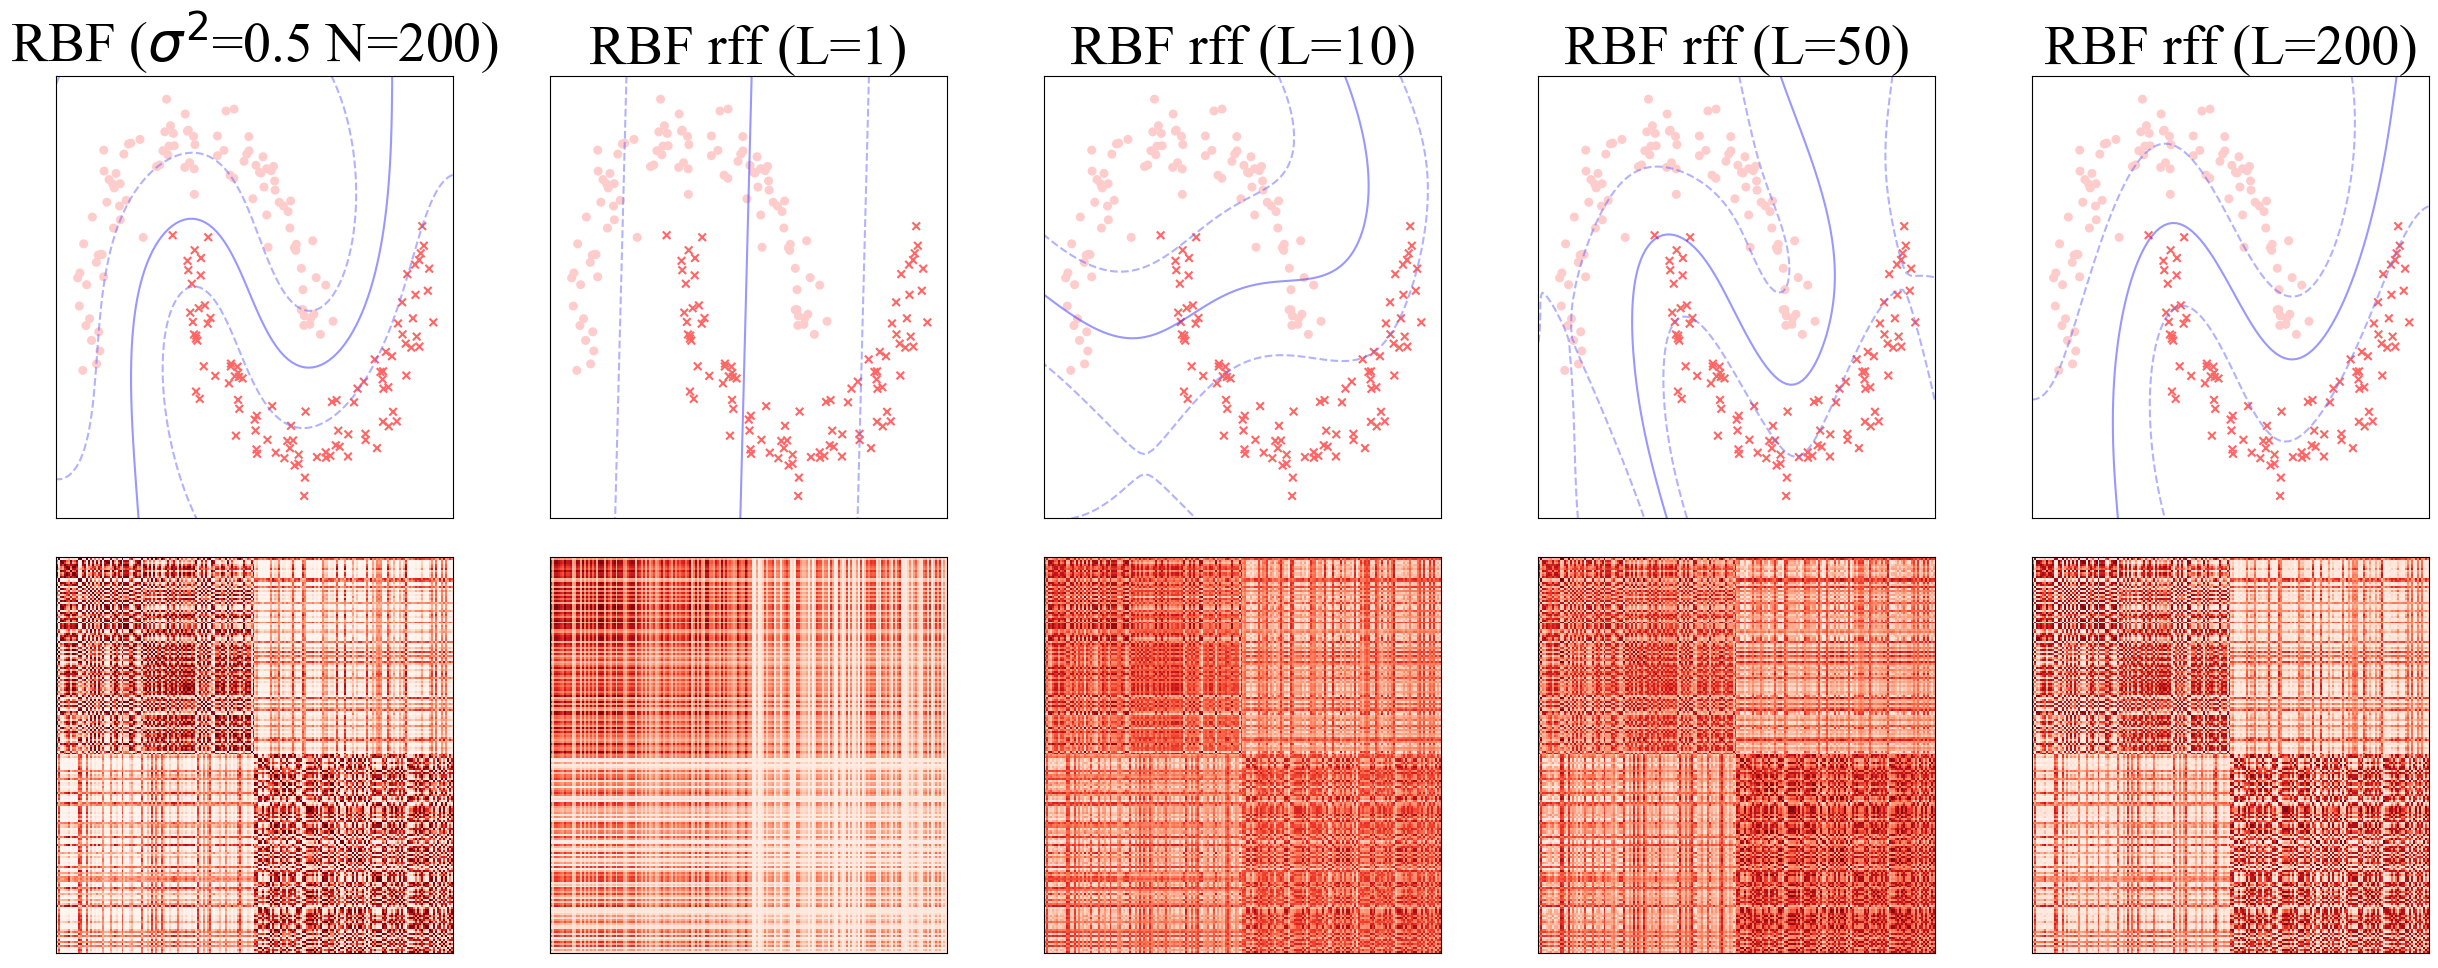
\includegraphics[width=\textwidth]{assets/rbf_rff_svm.png} 
    \caption{Radial basis kernel matrix ($\sigma^2=0.5$) and its random Fourier approximation (varying $L$) over moon dataset. Higher number of particles $L$ makes kernel matrix approximation better.}
    \label{fig:rbf_rff}
\end{figure}
\end{center} 

\section{Kernel Mean Embedding of Distributions}

\cite{muandetKernelMeanEmbedding2017} chapter 3 provides a really clear generalization from feature map over points $x\in\sX$ to measures over the measurable space $(\sX,\sF)$ where $\sF$ is sigma algebra of $\sX$. Let $\sH$ be a reproducing kernel Hilbert space with reproducing kernel $k$. Consider the mean map $\mu:\sP\to\sH$
\begin{align}
    \mu(\bbP)
        = \int k(x,\cdot) d\bbP(x)
\end{align}
and write $\mu_{\bbP} := \mu(\bbP)$. Intuitively, the mean map $\mu_{\bbP}$ is a representation of probability measure $\bbP$ in $\sH$. Not rigorously, we noticed that we can compute $\E_{\bbP}\pb{f(X)}$ as inner products in $\sH$,
\[
    \int f d\bbP
        = \int \inner{f}{k(x,\cdot)}_{\sH} d\bbP(x)
        = \inner{f}{\int k(x,\cdot)d\bbP(x)}_{\sH}
        = \inner{f}{\mu_{\bbP}}
\]
In effect, we are interchanging expectation and inner products, $\E\pb{\inner{f}{k(X,\cdot)}_{\sH}} = \inner{f}{\E\pb{k(X,\cdot)}}_{\sH}$.
\begin{lemma}
    \label{lemma:mean_embedding_reproducing_property}
    If $\E\pb{\sqrt{k(X,X)}} < \infty$, then $\mu_{\bbP} \in \sH$ and $\E_{\bbP}\pb{f(X)} = \inner{f}{\mu_{\bbP}}_{\sH}$ for all $f\in\sH$.
\end{lemma}
\begin{proof}
    For any $\bbP\in\sP$, define a linear functional $T_{\bbP}:\sH\to\R$ where $T_{\bbP}(f) = \E_{\bbP}\pb{f(X)}$ as the operation of taking expectation with respect to function $f\in\sH$ over $\bbP$. We show $T_{\bbP}$ is bounded (to use Rietz)
    \begin{align}
        |T_{\bbP}f|
            = |\E\pb{f(X)}|
            \leq \E\pb{|f(X)|}
            = \E\pb{ \left|  \inner{f}{k(X,\cdot)} \right| }
            \leq \E\pb{ \sqrt{k(X,X)} \norm{f}_{\sH} }
            < \infty
    \end{align}
    By Rietz representation theorem, exists $g\in\sH$ such that $T_{\bbP} f = \inner{f}{g}_{\sH}$. The choice of $f = k(x,\cdot)$ implies.
    \[
        g(x)
            = \inner{k(x,\cdot)}{g}_{\sH} 
            = T_{\bbP}\pb{k(x,\cdot)}
            = \int k(x,x') d\bbP(x')
            = \mu_{\bbP}(x)
    \]
    Therefore, $\mu_{\bbP}\in\sH$ is guaranteed by Rietz and we can re-write the Rietz's result and considered it as a reproducing property for $T_{\bbP}$, i.e. $\E\pb{f(X)} = \inner{f}{\mu_{\bbP}}_{\sH}$.
\end{proof}
In effect, what this lemma states is under some mild assumptions, the mean map $\mu_{\bbP}$ ends up in RKHS $\sH$ and that we can compute the expectation of any function in RKHS with respect to distribution $\bbP$ by computing inner product between the function $f$ and the mean map $\mu_{\bbP}$ in $\sH$. This is analogous to previous definition of a reproducing kernel, that the cannical feature map ends up in RKHS $k(x,\cdot) \in \sH$ and we can evaluate the evaluation functional as an inner product in RKHS, i.e. $\delta_x(f) = \inner{f}{k(x,\cdot)}_{\sH}$. 

Furthermore, we note that inner products of mean maps is expectation of kernel, i.e. for $X\sim\bbP,Y\sim\bbQ$,
\begin{align}
    \inner{\mu_{\bbP}}{\mu_{\bbQ}}_{\sH}
        = \E\pb{\mu_{\bbQ}(X)}
        = \E\pb{ k(X,Y) }
\end{align}
where we have used fact that evaluating the mean map at $x\in\sX$ computes the expectation of a kernel,
\begin{align}
    \mu_{\bbQ}(x)
        = \inner{\mu_{\bbQ}}{k(x,\cdot)}_{\sH}
        = \E\pb{k(x,Y)}
\end{align}
For appropriately chosen kernel, specifically a characteristic kernel, the mean map $\mu_{\bbP}$ completely characterizes a distribution. For example, the choice of $k(x,x') = e^{\inner{x}{x'}}$ implies that the mean embedding is the moment generating function $\mu_{\bbP} = \E\pb{e^{\inner{X}{\cdot}}}$.

\begin{definition}
    (Characteristic kernel) A kernel is characteristic if the map $\mu:\bbP\mapsto \mu_{\bbP}$ is injective
\end{definition}

A characteristic kernel ensures that the induced RKHS is rich enough to represent higher order momemts of $\bbP$. In particular, it ensures that $\norm{\mu_{\bbP}-\mu_{\bbQ}}_{\sH} = 0$ if and only if $\bbP=\bbQ$. As an example, Gaussian and Laplacian kernels are characteristic. Characteristic kernels are important when trying to distinguish distributions, might be less useful when trying to do predictive tasks with distributional data.

\begin{definition}
    (Universal kernel) A continuous positive definite kernel on compact metric space $\sX$ is universal if the corresponding RKHS $\sH$ is dense in $C(\sX)$, space of bounded continous functions over $\sX$.
\end{definition}

Universal kernel are characteristic kernels. See \cite{muandetKernelMeanEmbedding2017} for a classification of kernels.

We can derive empirical estimate of the mean map $\hat{\mu}_{\bbP} = \frac{1}{m}\sum_{i=1}^m k(\cdot,x_i)$ for $x_i \overset{iid}{\sim} \bbP$. 


\section{Maximum Mean Discrepancy}

The kernel mean embedding defines a natural metric for probability distributions, so called maximum mean discrepancy, as $\text{MMD}(\bbP,\bbQ)
= \norm{\mu_{\bbP}-\mu_{\bbQ}}_{\sH}$. In particular, evaluation can be deligated to kernels, 
\begin{align}
    \text{MMD}^2(\bbP,\bbQ)
        &= \inner{\mu_{\bbP}}{\mu_{\bbP}}_{\sH} + \inner{\mu_{\bbQ}}{\mu_{\bbQ}}_{\sH} - 2\inner{\mu_{\bbP}}{\mu_{\bbQ}}_{\sH} \\
        &= \E\pb{k(X,X')} + \E\pb{k(Y,Y')} - 2\E\pb{k(X,Y)}
\end{align}
where $X,X'\overset{iid}{\sim} \bbP$ and $Y,Y'\overset{iid}{\sim} \bbQ$. The unbiased quadratic $\sO(mn)$ estimate is given by
\begin{align}
    \widehat{\text{MMD}}_u^2(X,Y)
        = \frac{1}{m(m-1)} \sum_{i\neq j} k(x_i,x_j) + \frac{1}{n(n-1)} \sum_{i\neq j} k(y_i,y_j) - \frac{2}{mn} \sum_{i,j} k(x_i,y_j)
\end{align}
where $\bX = (X_1,\cdots,X_m) \overset{iid}{\sim}\bbP$ and $\bY = (Y_1,\cdots,Y_n) \overset{iid}{\sim} \bbQ$. Alternatively, we can consider maximum mean discrepancy as a class of integral probability metric over functions in the unit ball in RKHS $\sH$,
\begin{align}
    \text{MMD}(\bbP,\bbQ)
        = \sup_{f\in\sH:\; \norm{f}_{\sH}\leq 1} \pc{
            \int f d\bbP - \int f d\bbQ
        }
\end{align}
which is equivalent to the view of MMD as distance between kernel mean embeddings
\begin{align}
    \sup_{f\in\sH:\; \norm{f}_{\sH}\leq 1} \pc{
            \int f d\bbP - \int f d\bbQ
        }
        = \sup_{f\in\sH:\; \norm{f}_{\sH}\leq 1} \inner{f}{\mu_{\bbP}-\mu_{\bbQ}}_{\sH}
        = \norm{\mu_{\bbP} - \mu_{\bbQ}}_{\sH}
\end{align}
where optimal witness function is normalized difference of feature means $f^* = \mu_{\bbP}-\mu_{\bbQ}/\norm{ \mu_{\bbP}-\mu_{\bbQ} }_{\sH}$. Figure (\ref{fig:mmd_gauss_laplace_witness}) illustrates an empirical estimate of witness function, using kernels.



\begin{figure}[h!]
\begin{center} 
    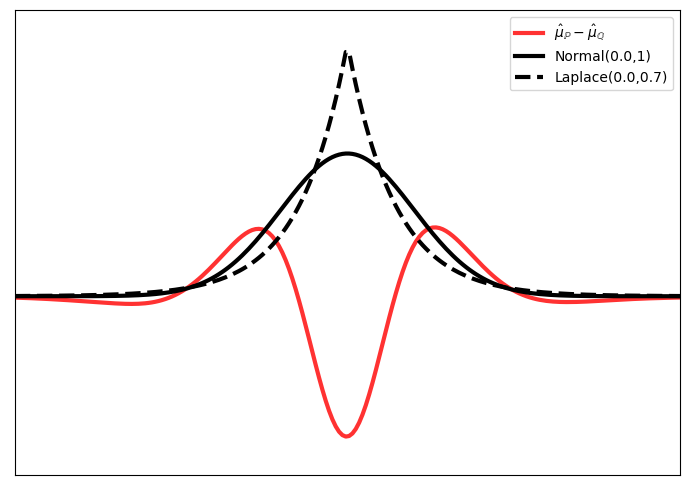
\includegraphics[width=3in]{assets/mmd_gauss_laplace_witness} 
    \caption{The unnormalized witness function $\hat{f^*} = \widehat{\mu_{\bbP}} - \widehat{\mu_{\bbQ}}$ where $\bbP \equiv \text{N}(0,1)$ is compared with $\bbQ \equiv \text{Lap}(0,\sqrt{.5})$. Both distribution has same mean and variance. The witness is computed from $4\times 10^4$ samples, using a Gaussian kernel with $\sigma^2=0.5$. The witness function is large whenever $\bbP-\bbQ$ is positive and small when $\bbP-\bbQ$ is large. This plot reproduces one figure in \cite{grettonKernelTwoSampleTest2012}.}
    \label{fig:mmd_gauss_laplace_witness}
\end{center}
\end{figure}

    

\begin{example}
    Consider $X_1\sim \sN(\mu_1,\Sigma_1), X_2\sim \sN(\mu_2,\Sigma_2)$. Let $\sH$ be RKHS with $k(x,y)=x^Ty$ as its reproducing kernel. We note that $\text{MMD}^2$ with linear witness is equivalent to difference in means,
    \begin{align}
        \text{MMD}^2(\bbP_{X_1},\bbP_{X_2})
            = \norm{\mu_{\bbP_{X_1}} - \mu_{\bbP_{X_2}}}_{\sH}^2
            = \norm{ k(\mu_1, \cdot) - k(\mu_2,\cdot) }_{\sH}^2
            = \norm{ k(\mu_1-\mu_2,\cdot) }_{\sH}^2
            = \norm{\mu_1 - \mu_2}_2^2
    \end{align}
    where $\mu_{\bbP_{X_1}}(x) = \E\pb{ k(x, X_1) } = x^T\E\pb{X_1}$ implies $\mu_{\bbP_{X_1}} = k(\mu_1, \cdot)$.
\end{example}





\section{Kernel Dependence Measures}

Intuitively, we can compare dependence between two random variables by computing the distance in a RKHS. \cite{grettonMeasuringStatisticalDependence2005} first proposes HSIC as Hilbert-Schmidt norm of covariance operator to measure dependence between two probability measures. \cite{muandetKernelMeanEmbedding2017} provides a good summary on the topic. \cite{grettonKernelMethodsMeasuring2005} provides good summary of several related kernel dependency measures like COCO and KMI. 

\subsection{Covariance Operators}

\cite{grettonNotesMeanEmbeddings2019} gives a pretty good introduction on covariance operators.

\begin{definition}
    (Hilbert-Schmidt operator) Let $\sG,\sF$ be separable Hilbert space and $\pc{f_j}_{j\in J}$, $\pc{e_i}_{i\in I}$ be orthonormal basis for $\sG$ and $\sF$, respectively. A Hilbert-Schmidt operator is a bounded operator $A:\sG\to\sF$ whose Hilbert-Schmidt norm $\norm{A}_{\text{HS}}$ is finite, 
    \begin{align}
        \norm{A}_{\text{HS}}^2 
            = \sum_{j\in J} \norm{A f_j}_{\sF}^2 
            = \sum_{i\in I}\sum_{j\in J} |\inner{A f_j}{e_i}_{\sF}|^2
    \end{align}
\end{definition}

Hilbert-Schmidt norm reduces to Frobenius norm when $\sG,\sF$ is $\R^n$ since $\norm{A}_{\text{HS}}^2 = \sum_{j=1}^n \norm{a_i}_2^2 = \sum_{i=1}^n \sum_{j=1}^n a_{ij}^2 = \norm{A}_{F}^2$. 
\begin{definition}
    (Space of Hilbert-Schmidt operators) The Hilbert-Schmidt operators from $\sG$ to $\sF$ with inner product defined below is a Hilbert space denoted as $\text{HS}(\sG,\sF)$.
    \begin{align}
        \inner{L}{M}_{\text{HS}} 
            = \sum_{j\in J} \inner{Lf_j}{Mf_j}_{\sF}
            = \sum_{i\in I}\sum_{j\in J} \inner{Lf_j}{e_i}_{\sF} \inner{Mf_j}{e_i}_{\sF}
    \end{align}
\end{definition}

Although the inner product is defined based on $(f_j)_{j\in J}$, it is in fact independent of the orthonormal basis chosen, as shown in \cite{grettonNotesMeanEmbeddings2019}. Additionally, we see that this inner product recovers the Hilbert-Schmidt norm, $\inner{L}{L}_{\text{HS}} = \sum_{j\in J} \inner{Lf_j}{Lf_j}_{\sF} = \sum_{j\in J} \norm{L f_j}_{\sF}^2 = \norm{L}_{\text{HS}}^2$. Another thing to note is that $\text{HS}(\sG,\sF) \simeq \sG\otimes \sF$.

\begin{definition}
    \label{def:tensor_product_hilbert}
    (Tensor product on Hilbert space) For $b\in\sG,a\in \sF$, the tensor product $a\otimes b$ is a rank-one operator from $\sG$ to $\sF$ defined as $(a\otimes b)(g) = \inner{g}{b}_{\sG} a$ for $g\in\sG$.
\end{definition}

Tensor product of spaces can be defined via a bilinear map fo the form $\sF\times\sG\to\R$ that satisfies the property of being linear in each input coordinate. We can define $(a\otimes b): \sG\times\sF\to\R$ with $(a\otimes b)(g,f) =\inner{g}{b}_{\sG}\inner{f}{a}_{\sF}$ and define the resulting tensor product space as $\sG\otimes \sF = \overline{\pc{a\otimes b}_{a\in\sF,b\in\sG}}$. Alternatively, we can define a map from $\sG$ to $\sF$ as previously and arrive at the same result. Intuitively, tensor product on function space generalizes outer product in Euclidean vector spaces. For example for $a,b\in\R^n$, we have $(ab^T)g = a(b^Tg)$, similar to definition (\ref{def:tensor_product_hilbert})

\begin{proposition}
    (Properties of tensor product \cite{grettonNotesMeanEmbeddings2019}) 
    \begin{enumerate}
        \item $\norm{a\otimes b}_{\text{HS}}^2 = \norm{a}_{\sF}^2 \norm{b}_{\sG}^2$ (and therefore $a\otimes b \in \text{HS}(\sG,\sF)$)
        \item $\inner{L}{a\otimes b}_{\text{HS}} = \inner{a}{Lb}_{\sF}$ for For $L\in\text{HS}(\sG,\sF)$ ($L=u\otimes v$ implies $\inner{u\otimes v}{a\otimes b}_{\text{HS}} = \inner{u}{a}_{\sF} \inner{v}{b}_{\sG}$)
    \end{enumerate}
\end{proposition}

The take-away is that tensor products are Hilbert-Schmidt operators and we can evaluate HS inner product of two tensor products as multiple of two inner products in $\sG,\sF$.

\begin{definition}
    (Cross-covariance operator) Let $(X,Y)$ be random variables over $\sX\times\sY$ and $(\sF,k,\phi)$ and $(\sG,l,\psi)$ be RKHS, its reproducing kernel and feature map, respectively. $\widetilde{C}_{XY}:\sG\to\sF$ is called the (uncentered) cross-covariance operator
    \begin{align}
        \widetilde{C}_{XY}
            = \E\pb{ \phi(X) \otimes \psi(Y) }
    \end{align}
    The corresponding centered covariance operator is 
    \begin{align}
        C_{XY} 
            = \E\pb{ (\phi(X)-\mu_X)\otimes (\psi(Y)-\mu_Y) }
            = \widetilde{C}_{XY} - \mu_{X} \otimes \mu_{Y}
    \end{align}
    where $\mu_X = \E\pb{\phi(X)}, \mu_Y = \E\pb{\psi(Y)}$ are mean embeddings of $\bbP_X,\bbP_Y$.
\end{definition}


Intuitively, we can think of $\phi(X)\otimes \psi(Y)$ as a random variable in space of operators $\text{HS}(\sG,\sF)$ or in the tensor product feature space $\sG\otimes \sF$. The definition generalizes finite dimensional (uncentered) covariance matrix $\E\pb{XY^T}$ to be the corresponding covariance matrix in the tensor product feature space. Equivalently, we can consider cross-covariance operator as mean embedding of $\bbP_{XY}$ in $\sG\otimes\sF$ induced by product kernel $v((x,y),(x',y') = k(x,x')l(y,y')$, i.e. $\widetilde{C}_{XY} = \mu_{\bbP_{XY}}$. 

\begin{lemma}
    If $\E\pb{\norm{\phi(X)\otimes \psi(Y)}_{\text{HS}}} < \infty$, then $\widetilde{C}_{XY}\in\text{HS}(\sG,\sF)$ and $\widetilde{C}_{XY}$ uniquely satisfies
    \begin{align}
        \label{eq:crosscovariance_operator_riesz}
        \inner{\widetilde{C}_{XY}}{A}_{\text{HS}} 
            = \E\inner{\phi(X)\otimes \psi(Y)}{A}_{\text{HS}}
    \end{align}
    for any $A \in \text{HS}(\sG,\sF)$.
\end{lemma}

\begin{proof}
    Detail in \cite{grettonNotesMeanEmbeddings2019}. Define linear operator $T_{XY}: \text{HS}(\sG,\sF) \to\R$ as $T_{XY}(A) \mapsto \E\inner{\phi(X)\otimes \psi(Y)}{A}_{\text{HS}}$ and show it is bounded. Use Riesz representation theorem to guarantee existence of $\widetilde{C}_{XY}$ satisfying the equation and show that it has the form defined previously.
\end{proof}

Again, we can consider (\ref{eq:crosscovariance_operator_riesz}) as exchanging expectation and inner products over $\text{HS}(\sG,\sF)$. In particular, if we let $A=f\otimes g$, then we can use properties of tensor product and the previous lemma and get
\begin{align}
    \inner{f}{\widetilde{C}_{XY}g}_{\sF}
        &= \inner{\widetilde{C}_{XY}}{f\otimes g}_{\text{HS}} 
        = \E\inner{\phi(X)\otimes\psi(Y)}{f\otimes g}_{\text{HS}} 
        = \E\pb{ \inner{f}{\phi(X)}_{\sF} \inner{g}{\psi(Y)}_{\sG} } \\
        &= \E\pb{ f(X)g(Y) }
        = \cov(f(X),g(Y))
\end{align}

This is used to show HSIC as IPM with two witness functions $f\in\sF,g\in\sG$. From this result, we can compute the application of the covariance operator to $g\in\sG$ with an expectation over kernels 
\begin{align}
    (C_{XY} g)(y')
        = \inner{l(\cdot, y')}{C_{XY}g}_{\sG}
        = \int f(X) l(Y,y') d\bbP_{XY}
\end{align}
We can visualize $C_{XY}g \in \sF$ to get an intuition about $C_{XY}$.


\subsection{Hilbert-Schmidt Independence Criterion}

\cite{grettonMeasuringStatisticalDependence2005} uses Hilbert-Schmidt norm of (centered) covariance operator to measure dependence,
\begin{align}
    \text{HSIC}(\sF,\sG,\bbP_{XY})
        = \norm{\widetilde{C}_{XY}}_{\text{HS}}
        = \norm{ C_{XY} - \mu_X \otimes \mu_{Y} }_{\text{HS}}
\end{align}
Equivalently, we can consider $\text{HSIC}$ as MMD between kernel embedding of joint $\bbP_{XY}$ with that of product of marginals $\bbP_X\bbP_Y$ over the tensor product feature space $\sG\otimes\sF$,
\begin{align}
    \text{HSIC}(\sF,\sG,\bbP_{XY})
        = \text{MMD}(\bbP_{XY},\bbP_X\bbP_Y)
        = \norm{ \mu_{\bbP_{XY}} - \mu_{\bbP_X\bbP_Y} }_{\sG\otimes\sF}
\end{align} 

\begin{proposition}
    (HSIC and Independence) $\text{HSIC}(\sF,\sG,\bbP_{XY})=0$ if and only if $X\dperp Y$.
\end{proposition}

Computation of HSIC can be delegated to kernels again (see \cite{grettonNotesMeanEmbeddings2019} for detailed derivation), implying that we can compute a measure of dependence between $X$ and $Y$ via expectation over kernels without needing to perform density estimation. 
\begin{align}
    \text{HSIC}(\sF,\sG,\bbP_{XY})
        &= \E_{X,Y} \E_{X',Y'} k(X,X')l(Y,Y')
            + \E\pb{k(X,X')}\E\pb{k(Y,Y')} \\ 
        &\quad -2 \E_{X,Y} \pb{ \E\pb{k(X,X')} \E\pb{l(Y,Y')} }
\end{align}
Given samples $Z = \pc{(x_i,y_i)}_{i=1}^n \overset{iid}{\sim} \bbP_{XY}$, we have a simple biased estimate,
\begin{align}
    \widehat{\text{HSIC}}_b^2(\sF,\sG,Z)
        = \frac{1}{n^2} \tr(\widetilde{\bK}\widetilde{\bL})
        = \frac{1}{n^2} \tr(\bK\bH\bL\bH)
\end{align}
where $\widetilde{\bK},\widetilde{\bL}$ are centered kernel matrices computed from kernels $k,l$ and $\bH$ is the centering matrix (Refer to example (\ref{exampe_centering_matrix}) for centering in feature space). The last equality given by fact that $\bH$ is indempotent and cyclic property of trace. \cite{songFeatureSelectionDependence2012a} derived an unbiased $\sO(n^2)$ estimator,
\begin{align}
    \text{HSIC}^2(\sF,\sG,Z)
        &= \frac{1}{n(n-3)} \pb{
            \tr(\widetilde{\bK}\widetilde{\bL}) + 
            \frac{ \mathbf{1}^T \widetilde{\bK} \mathbf{1} \mathbf{1}^T \widetilde{\bL} \mathbf{1} }{ (n-1)(n-2) } -
            \frac{2}{n-2} \mathbf{1}^T \widetilde{K}\widetilde{L}\mathbf{1} 
        }
\end{align}


\begin{example}
    \label{exampe_centering_matrix}
    (Centering Matrix \cite{scholkopfNonlinearComponentAnalysis1998} A.1) Given $\varphi$ and a set of observations $x_1,\cdots,x_n$, we might want to centered features $\widetilde{\varphi}(x_i) = \varphi(x_i) - \overline{\varphi}$ where $\overline{\varphi} = \frac{1}{n}\sum_{i=1}^n \varphi(x_i)$ is the centroid. We want to find centered kernel matrix $\widetilde{\bK}$ such that $\widetilde{\bK}_{ij} = \inner{\widetilde{\varphi}(x_i)}{\widetilde{\varphi}(x_j)}_{\sH}$. Note,
    \begin{align}
        \widetilde{\bK}_{ij}
            &= \inner{\widetilde{\varphi}(x_i)}{\widetilde{\varphi}(x_j)}_{\sH} \\
            &= \inner{ \varphi(x_i) - \frac{1}{n}\sum_{s=1}^n \varphi(x_s) }{ \varphi(x_j) - \frac{1}{n}\sum_{t=1}^n \varphi(x_t) }_{\sH} \\ 
            &= k(x_i,x_j) - \frac{1}{n} \sum_{s=1}^n k(x_s, x_j) - \frac{1}{n} \sum_{t=1}^n k(x_t, x_i) + \frac{1}{n^2} \sum_{s=1}^n \sum_{t=1}^n k(x_s, x_t) \\ 
            &= \bK_{ij} - (\mathbf{1}_n \bK)_{ij} - (\bK\mathbf{1}_n)_{ij} + (\mathbf{1}_n \bK \mathbf{1}_n)_{ij} \\ 
            &= (( \bI - \mathbf{1}_n ) \bK ( \bI - \mathbf{1}_n ))_{ij} \\
            &= (\bH\bK\bH)_{ij}
    \end{align}
    where $\mathbf{1}_n \in \R^{n\times n}$ defined as $\mathbf{1}_n = \frac{1}{n}\mathbf{1}\mathbf{1}^T$. Therefore, $\widetilde{\bK} = \bH \bK \bH$ where $\bH = \bI - \mathbf{1}_n$.
\end{example}



    
\begin{example}
    (2D Gaussian) Let $X\sim \sN(\mu, \Sigma)$ over $\R^2$ where $\mu=\mathbf{1}$, $\Sigma=\bI_2$. Consider $A \in \R^{2\times 2}$ where $a_1,a_2$ are rows of $A$. Let $(y_1,y_2) := Y = AX$ where $Y\sim \sN(A\mu, A\Sigma A^T)$. We want to find coefficients of linear map that makes the transformed variables independent subject to constraint that the $\sum_{j} a_ij = 1$ for $i=1,2$ to avoid degenerate zero mapping solution,
    \begin{align}
        \label{eq:hsic_2d_gaussian_optimization}
        \min_{a_1,a_2} \text{HSIC}_k(a_1x, a_2x) - \lambda \norm{ A\mathbf{1}-\mathbf{1} }^2
    \end{align}
    Note $y_1\dperp y_2$ if and only if $A\Sigma A^T = I$, which is what we observe in simulation. See Figure (\ref{fig:hsic_2d_gaussian})
\end{example} 



\begin{figure}[h!]
    \begin{center} 
        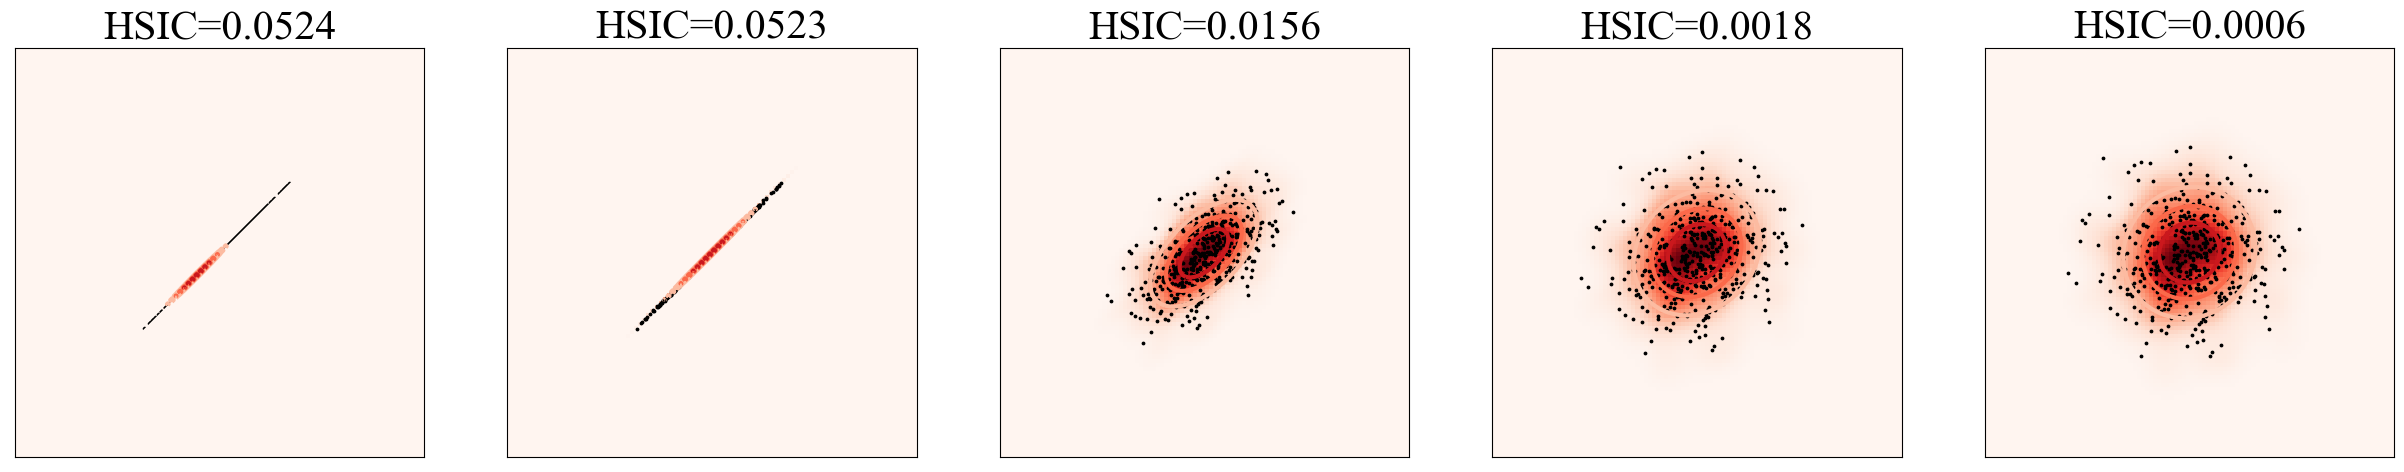
\includegraphics[width=\textwidth]{assets/hsic_2d_gaussian} 
        \caption{Use stochastic gradient descent to optimize for (\ref{eq:hsic_2d_gaussian_optimization}) where we have used RBF kernel with bandwidth chosen using median heuristic. We plotted transformed point by the linear mappings and its estimated density using Gaussian KDE. We also plotted contours of density of $Y$. Note as optimization progresses, the transformed points look as if they are sampled from an isotropic Gaussian.}
        \label{fig:hsic_2d_gaussian}
    \end{center}
    \end{figure}
    


 

\newpage
\printbibliography 




\end{document}